\section{The Heisenberg model}

The Heisenberg model is similar to the Ising model. We have lattice points on a line or a grid with a spin value, affected by a external field. In contrast with the Ising model, however, the Heisenberg model introduces coupling in all directions: $x$, $y$ and $z$. We will look at the so called XXX model, where the coupling strength is the same in each direction. So we expand our Ising Hamiltonian accordingly:

\begin{equation}
  H(\boldsymbol{\sigma}) =J\sum_{\langle i,j\rangle} \left ( \sigma^x_i\sigma^x_j + \sigma^y_i\sigma^y_j + \sigma^z_i\sigma^z_j\right) + L \sum_j \sigma^z_j \; ,
  \label{eq:heisen_hamiltonian}
\end{equation}

The idea behind construction of the Hamiltonian matrix is the same as for Ising, where we only need to extend \ref{eq:coupling_spin} by replacing the Pauli-z spin matrix with Pauli-x and Pauli-y accordingly.

\subsection{Eigenvalues through diagonalization}

Takeing the two-particle one-dimensional heisenberg model we set the external field strength to $L = 1$ and vary the couplng strength from $J = -1$ to $J= 1$. The energy levels then evolve as:

\begin{figure}[H]
  \begin{center}
    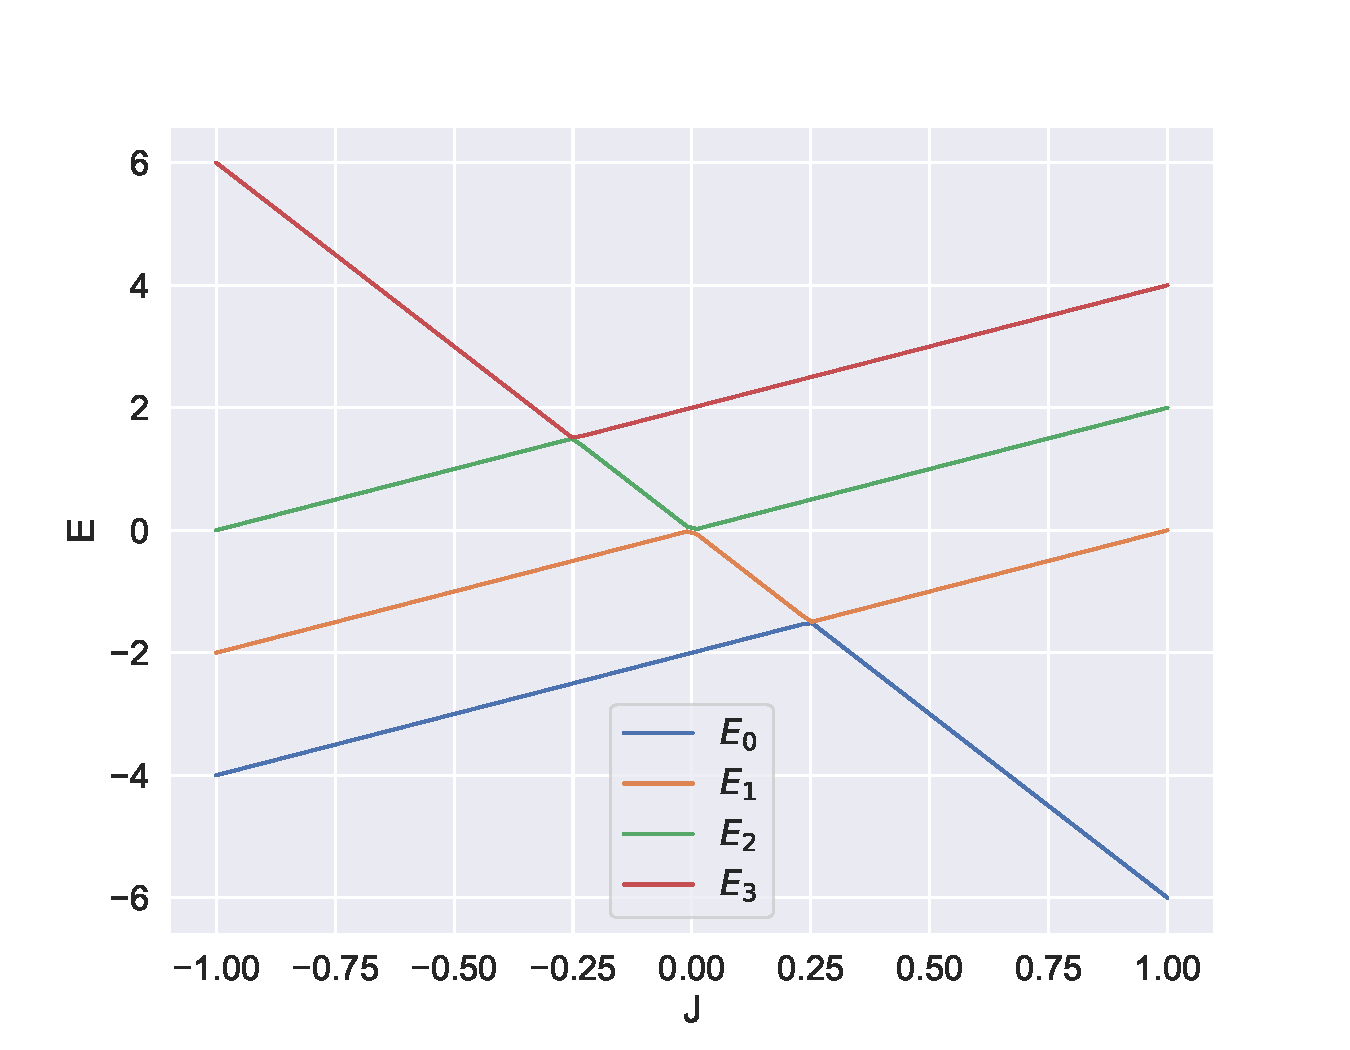
\includegraphics[width=0.95\textwidth]{Figures/Plots/Heisen/heisen_eig_21}
  \end{center}
  \caption{The eigenvalues of the two-particle Heisenberg Hamiltonian matrix with $L = 1$.}
\end{figure}

For a two-dimensional Heisenberg model we up the particle count to four to be able to make a $2\times 2$ lattice. We then get:


\begin{figure}[H]
  \begin{center}
    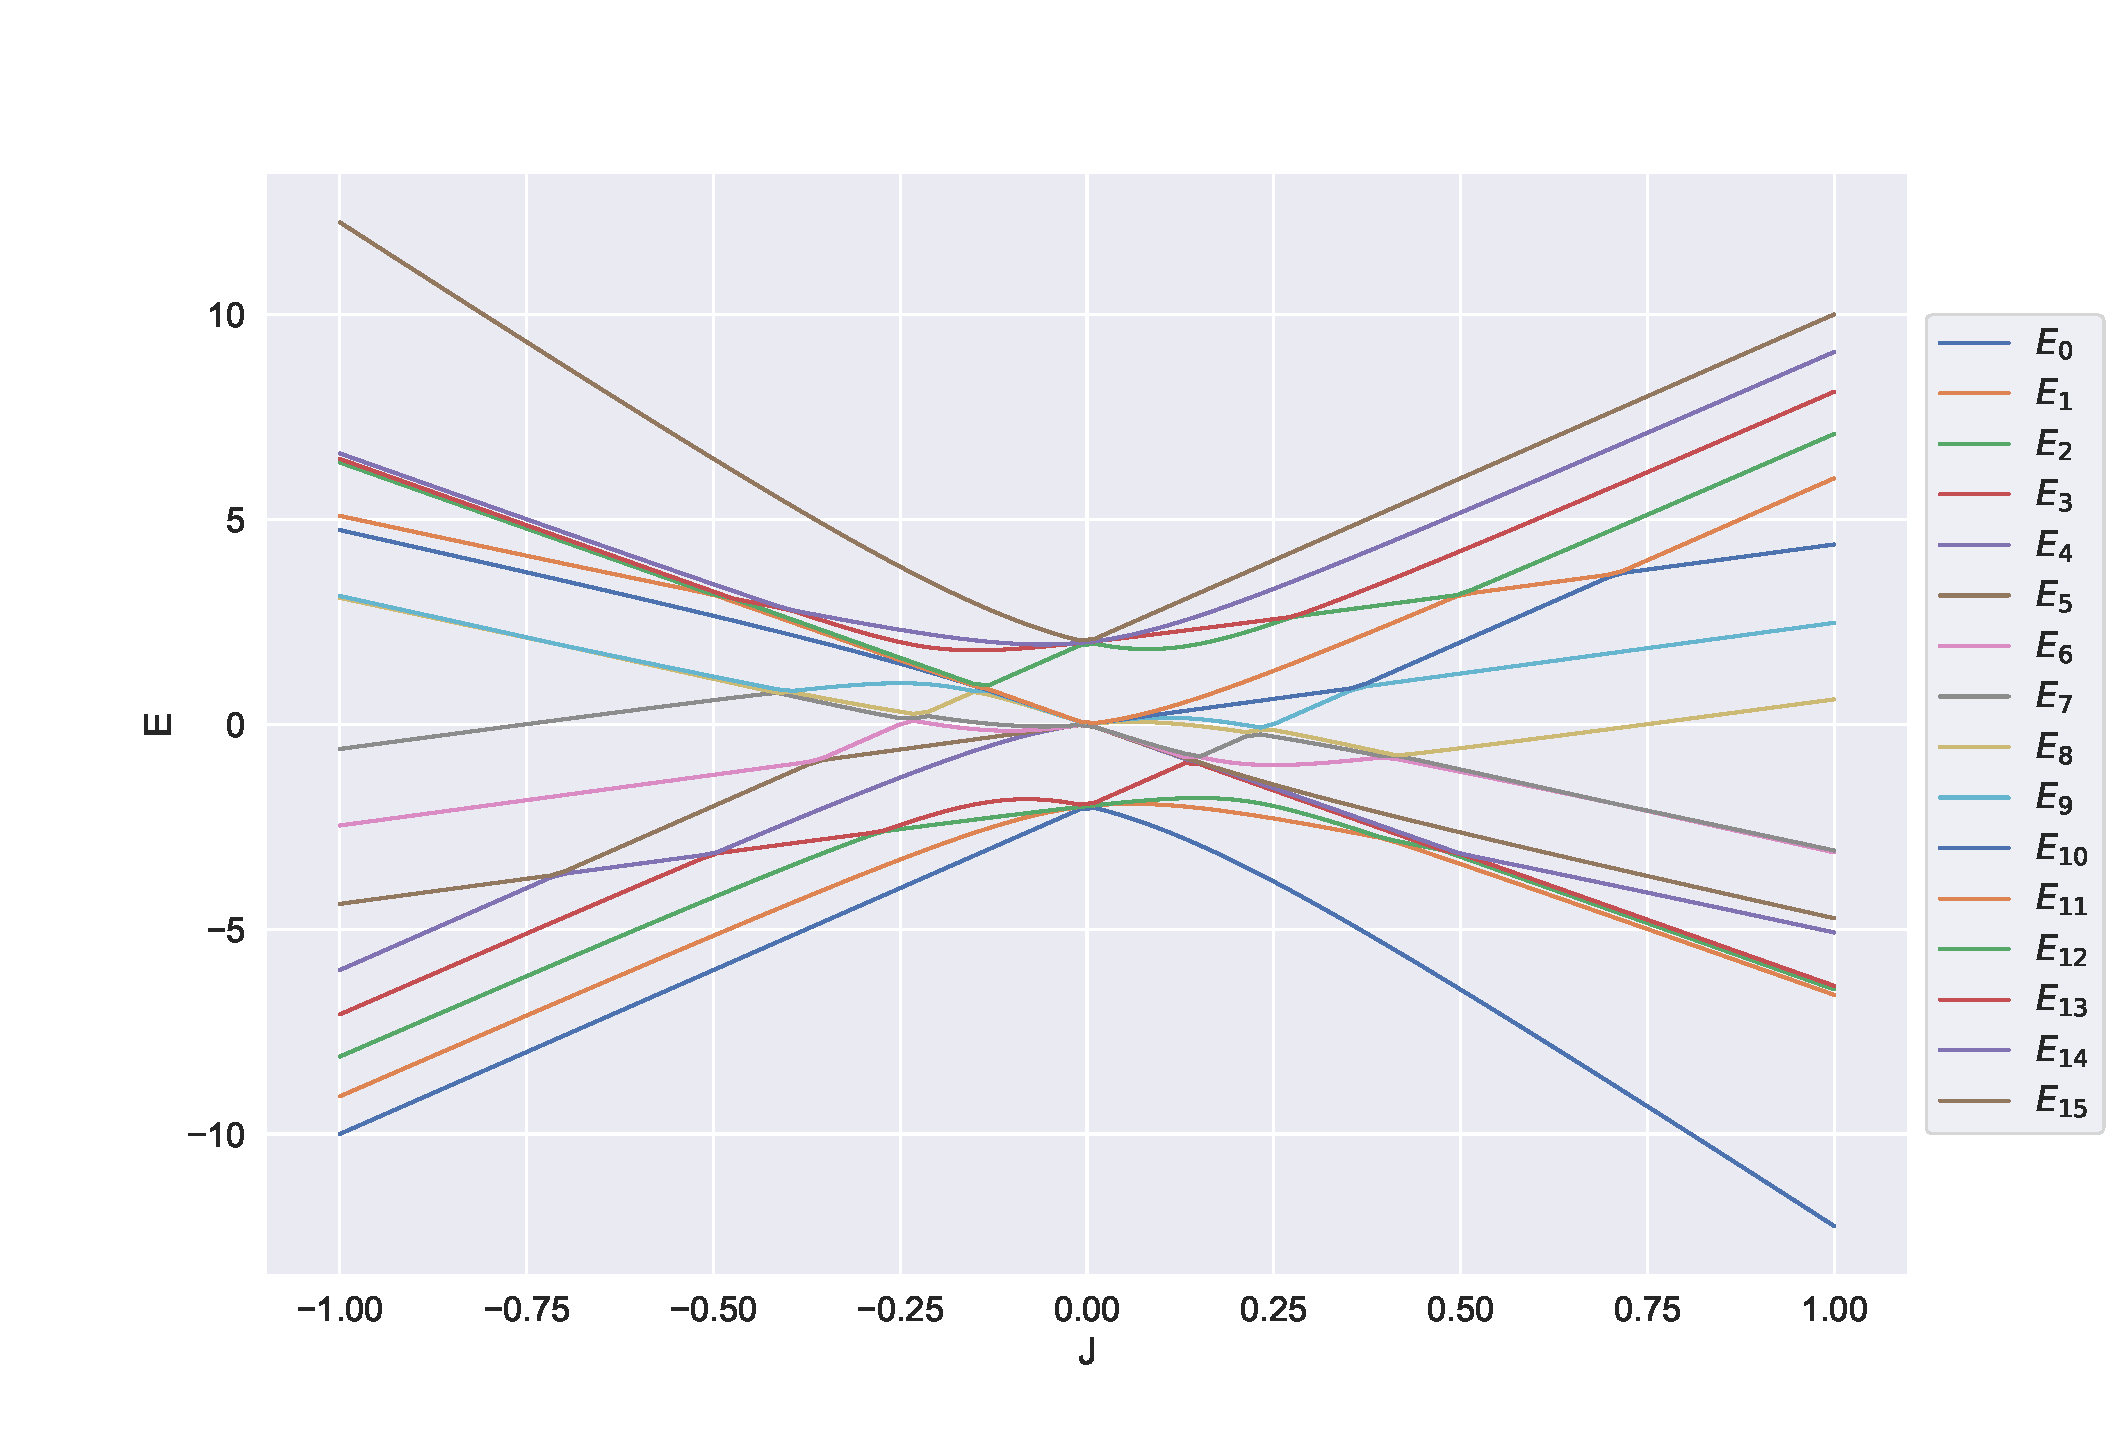
\includegraphics[width=0.95\textwidth]{Figures/Plots/Heisen/heisen_eig_22}
  \end{center}
  \caption{The eigenvalues of the four-particle two-dimensional Heisenberg Hamiltonian matrix with $L = 1$.}
\end{figure}


